% !TeX root = text.tex
\chapter{software}
Tento laserový projektor se skládá ze dvou částí. Jednou je software pro řízení galvanometrů a druhou je software pro interakci s uživatelem.
\fxnote{TODO: zkrátit věty}

O řízení galvanometrů se stará program lasershow, který je psaný v jazyce c++ pro maximální rychlost. Tento program běží na pozadí a čeká na příkazy od programů určených k interakci s uživatelem. Na tento program se zaměřuje kapitola lasershow. \fxnote{TODO: odkaz}

Dále jsou tu programy, které se starají o interakci s uživatelem. Tyto programy přijímají příkazy od uživatele a posílají je programu lasershow. Navíc od lasershow získávají výstup, který následně zprostředkovávají uživateli; důkladněji popsáno v kapitole \ref{sec:comms}.

Mezi tyto programy patří programy UI, web\_ui a discord\_bot. Program UI spravuje OLED displej, přijímá od uživatele vstup rotačním enkodérem a je psaný v c++ pro jednodušší interakci s hardwarem. Program web\_ui využívá runtime Node.js, ve kterém je nenáročné vytvořit http server dostupný z lokální sítě. \fxnote{(A)?} Program discord\_bot, také využívající Node.js, přijímá příkazy z chatovací aplikace discord a je přístupný i přes internet.

Nakonec je tu program wifi\_manager, ten spravuje wifi připojení RPi, je psaný v Node.js a komunikuje s programy, které interagují s uživatelem stejně jako program lasershow.

\section{komunikace mezi programy} \label{sec:comms}
Všechny tyto programy jsou propojeny síťovými sockety zprostředkovanými knihovnou ZeroMQ, která nabízí frontu\footnote{Ve frontě jsou zprávy seřazeny od té nejdříve odeslané.} zpráv, bez potřeby samostatně běžícího brokeru.\fxnote{TODO: divna jednicka}

Tato knihovna je využita k vytvoření dvou socketů, jedním lasershow přijímá příkazy od uživatele prostřednictvím ostatních programů (vstupní socket na portu 5557, viz obr. \ref{fig:tcp5557}) a do druhého posílá informace ostatním programům (výstupní socket na portu 5556, viz obr. \ref{fig:tcp5556}), aby je zprostředkovaly uživateli. Do prvního zmíněného posílají progamy interagující s uživatelem příkazy pro programy lasershow a wifi\_manager. Do druhého posílá lasershow informace o stavu a změnách nastavení  a také wifi\_manager informace o stavu a změnách v nastavení WiFi.

Příkazy pro programy lasershow a wifi\_manager vypadají následovně
\fxnote{TODO: příklady příkazů pro lasershow a wifi\_manager z \url{https://github.com/phuid/laser_projector/blob/master/README.md}}
\fxnote{TODO: příklady status infos od lasershow a wifi\_manager z \url{https://github.com/phuid/laser_projector/blob/master/README.md}}

\begin{figure}[!htb]
  \centering
  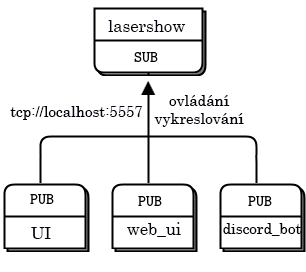
\includegraphics[width=0.5\textwidth]{img/tcp5557.png}
  \caption{\label{fig:tcp5557}komunikace mezi programy vstupním socketem na portu 5557}
\end{figure}
\begin{figure}[!htb]
  \centering
  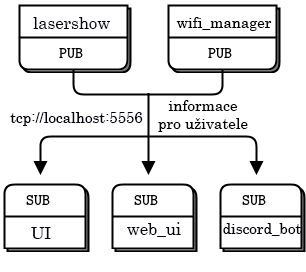
\includegraphics[width=0.5\textwidth]{img/tcp5556.png}
  \caption{\label{fig:tcp5556}komunikace mezi programy výstupním socketem na portu 5556}
\end{figure}

\section{lasershow}

Program lasershow je psaný v jazyce c++, který je kompilovaný a obecně považovaný za jeden z nejrychlejších jazyků. Druhé zmíněné se hodí, jelikož chceme vykreslovat co možná nejrychleji.

Tento program zaregistruje vstupní TCP socket na portu 5557 a knihovnou ZeroMQ se na něm přihlásí k odběru zpráv, které do něj publikují ostatní programy. Zárověn podobně zaregistruje výstupní socket na portu 5556, do kterého později bude posílat zprávy pro programy, které interagují s uživatelem.

Následně se připojí k DAC a čeká na zprávy od ostatních programů. Jakmile zprávu obdrží, zpracuje ji a pokud je požadována změna nastavení, okamžitě ji provede a aktuální nastavení si uloží do souboru, jestliže je požadováno vykreslení obrazu ze souboru, začne obraz vykreslovat. Při tom průběžně posílá informace o stavu vykreslování do výstupního socketu. I při vykreslování obrazu tento program zpracovává zprávy a pokyny ze vstupního socketu.

Program byl původně převzat z projektu \url{https://github.com/tteskac/rpi-lasershow}\footnote{staženo 28.~12.~2023}, následně byl ale přepsán skoro ve všech ohledech a z původního programu zbylo asi 20 řádků.
\fxnote{TODO: odkud jsem to vzal a prepsal a jak moc jsem toho udelal a s jakymy vysledky}

\fxnote{TODO: diagram programu}

\fxnote{TODO: priklad zmq}\

\lstinputlisting[language=c++, style=code]{code_examples/zmq_server.cpp}
\lstinputlisting[language=c++, style=code]{code_examples/zmq_client.cpp}

\section{UI}

Program UI je také psaný v jazyce c++ a využívá knihovnu WiringPi, která umožňuje jednoduchou komunikaci s GPIO piny Raspberry Pi. Tento program ovládá OLED displej, který je připojený na Raspberry Pi pomocí rozhraní I2C, a přijímá vstup od uživatele čtením rotačního enkodéru s tlačítkem.

Program se při začátku exekuce pomocí knihovny ZeroMQ přihlásí ke vstupnímu socketu a k odběru zpráv z výstupního TCP socketu, kam publikuje zprávy o stavu vykreslování program lasershow. Dále si pomocí knihovny wiringPi zaregistruje zpracovávání přerušení z enkodéru a tlačítka na něm a čeká buď na interakci s uživatelem, který by skrz něj poslal zprávy programu lasershow, nebo na zprávy od lasershow, které by zobrazil uživateli.

\fxnote{TODO: diagram programu}

\section{web\_ui}

Narozdíl od předchozích dvou zmiňovaných programů je program web\_ui psaný v jazyce javascript, ten nepatří mezi nejrychlejší, ale díky runtime Node.js a knihovnám http a formidable v něm bylo časově nenáročné vytořit http web server.

Tento server běží na portu 3000 a je dostupný z lokální sítě (tzn. přímo z\ Raspberry Pi na adrese http://localhost:3000 nebo z jakéhokoliv zařízení na stejné lokální síti na adrese http://IP\_ADRESA\_RPI:3000).
Program je využíván pro jednoduchou interakci s uživatelem, který může pomocí webového prohlížeče ovládat laserový projektor pár kliknutími i zadávat vlastní příkazy klávesnicí.

\fxnote{TODO: příklad http serveru}
\lstinputlisting[language=JavaScript, style=code]{code_examples/http_static_files.js}

Stejně jako program UI za pomoci knihovny ZeroMQ tento program odebírá z výstupního socketu zprávy o průběhu vykreslování od programu lasershow a odesílá mu pokyny uživatele na vstupní socket.

\fxnote{TODO: příklad přihlášení k socketům v js}

\fxnote{TODO: xterm + ssh}

\section{discord bot}

Posledním programem, který je využíván k interakci s uživatelem je discord\_bot, který je také psaný v jazyce javascript v runtime Node.js, stejně jako předchozí programy se přihlásí k socketům knihovnou zmq, ale na rozdíl od nich tento program může interagovat s uživatelem přes internet ať už je kdekoliv na světě.
Pomocí knihovny discord.js se přihlásí k předem vytvořenému bot účtu, který může na předem vytvořeném discord serveru čekat na zprávy od uživatele, ty posílat do vstupního socketu a posílat uživateli zpětnou vazbu, kterou příjme z výstupního socketu.

\section{wifi\_manager}

V rámci této práce byl vyvinut ještě jeden program, který se přímo nepodílí ani na projekci, ani na interakci s uživatelem.

Program wifi\_manager je také napsaný v jazyce JavaScript s využitím runtime Node.js. Registruje se ke stejným socketům jako lasershow, přijímá příkazy týkající se nastavení WiFi na Raspberry Pi TCP socketem na portu 5557 a odesílá zpětnou vazbu na TCP socket s portem 5556.

\fxnote{TODO: jak se komunikace s lasershow odlisuje od wifi\_managera}

\fxnote{TODO: ukazka(idk what)}

Hlavním úkolem tohoto programu je správa a konfigurace WiFi připojení na Raspberry Pi. Přijímá příkazy od ostatních programů a nastavuje WiFi parametry na základě těchto příkazů. Tím umožňuje uživatelům snadno a pohodlně nastavit WiFi připojení na svém zařízení.

Stejně jako lasershow, wifi\_manager také posílá zpětnou vazbu ostatním programům, aby informoval o stavu a změnách v nastavení WiFi. Tímto způsobem je zajištěna komunikace a synchronizace mezi všemi programy v laserovém projektoru.

Celkově wifi\_manager přispívá k plynulému a efektivnímu provozu laserového projektoru tím, že umožňuje snadnou správu a konfiguraci WiFi připojení na Raspberry Pi.